\newpage
\section*{Appendix A: List of Variables}
\label{sec:appendix_a}

Table~\ref{tb:variables_list} presents the complete list of variables in the dataset and their description:

\begin{table}[H]
    \small
    \centering
    \makebox[\textwidth][c]{
    \begin{tabularx}{1.1\textwidth}{ >{\hsize=0.7\hsize}X >{\hsize=1.3\hsize}X}
    \hline
    \textbf{Variable} & \textbf{Description}\\
    \hline
    fem\_empl\_rate & Employed women (15-64) / Total women (15-64)\\
    population & Residents on January $1^{st}$\\
    unempl\_rate & Unemployed (15-64) / Labor force (15-64)\\
    \textbf{part\_rate} & Labor force (15-89) / Population (15-89)\\
    empl\_rate & Employed (15-64) / Labor force (15-64)\\
    \textbf{empl\_growth} & Annual growth of employed population\\
    inact\_rate & Inactive (15-64) / Population (15-64)\\
    \textbf{fem\_edu\_rate} & Women 20+ with tertiary education\\
    \textbf{male\_edu\_rate} & Men 20+ with tertiary education\\
    \textbf{service\_empl\_rate} & Workers in service (15-64) / All workers\\
    \textbf{GDP} & Gross Domestic Product at market prices per person\\
    \textbf{n\_large\_comp} & Local units with 250+ employees / Active population (in thousands)\\
    \textbf{n\_self\_empl} & Number of self-employed / Active population\\
    young\_neet & 15-29 not in employement, education or training / 15-29 people\\
    \textbf{fem\_house\_rate} & Inactive women / Children aged 0-2\\
    \textbf{foreign\_rate} & Foreigners / Total population\\
    n\_members\_family & Average numer of members per family\\
    elderly\_in\_care & 65+ in home or interated care services\\
    house\_price & Average price per housing (€/$m^2$)\\
    fertility\_rate & Live births per 1000 residents\\
    first\_birth\_maternal\_age & Average age at first childbirth\\
    avg\_children\_per\_woman & Total fertility rate (TFR)\\
    dependency\_rate & Non-working / Working-age population\\
    ageing\_index & 65+ / 0-14 population\\
    net\_migration\_rate & Net migration per 1000 residents\\
    adj\_net\_migration\_rate & Migration adjusted for natural change\\
    area\_km2 & Total surface area\\
    public\_transport\_supply & Public transport supply per capita\\
    internet\_coverage\_rate & \% on households with high-speed internet\\
    graduate\_mobility\_rate & Net migration of graduates (25-39)\\
    green\_m2\_capita & Green space per capita in provincial capitals\\
    eco\_urban\_index & Environmental performance score\\
    \textbf{per\_capita\_public\_expenditure} & Municipal spending per 0-2 years old\\
    ecec\_participation & \% of 0-2 years old using early childhood services\\
    \textbf{coverage} & Number of available children services / Children aged 0-2\\
    urban\_type & 1: Urban, 2: Intermediate, 3: Rural\\
    \textbf{per\_capita\_user\_contribution} & Per-child user spending (€ per 0-2 years old)\\
    \textbf{advanced\_business\_empl} & Employees in advanced business services per active population\\
    lifelong\_learn & \% of population aged 25-64 in lifelong learning\\
    startup\_ratio & Innovative startups per 1000 corporations\\
    \textbf{fem\_maj\_empl\_rate} & Workers in Education and Health and Social Care / All workers\\
    \hline
    \end{tabularx}
    }
    \caption{List of numerical variables present in the data. Highlighted rows show computed variables, not directly taken.}
    \label{tb:variables_list}
\end{table}

\newpage
Figure \ref{fig:scatterplot} reports a pairwise scatterplot matrix for the outcome ($\texttt{fem\_empl\_rate}$) and ECEC variables. The diagonal panels show the marginal distributions of each variable, while the lower panels display the corresponding bivariate relationships and the higher ones displays correlation values. Observations are colored by Italian macro-area ($\texttt{rip\_name}$), highlighting geographic heterogeneity and potential North–South differences in both covariate distributions and associations with female employment:

\begin{figure}[h]
    \centering
    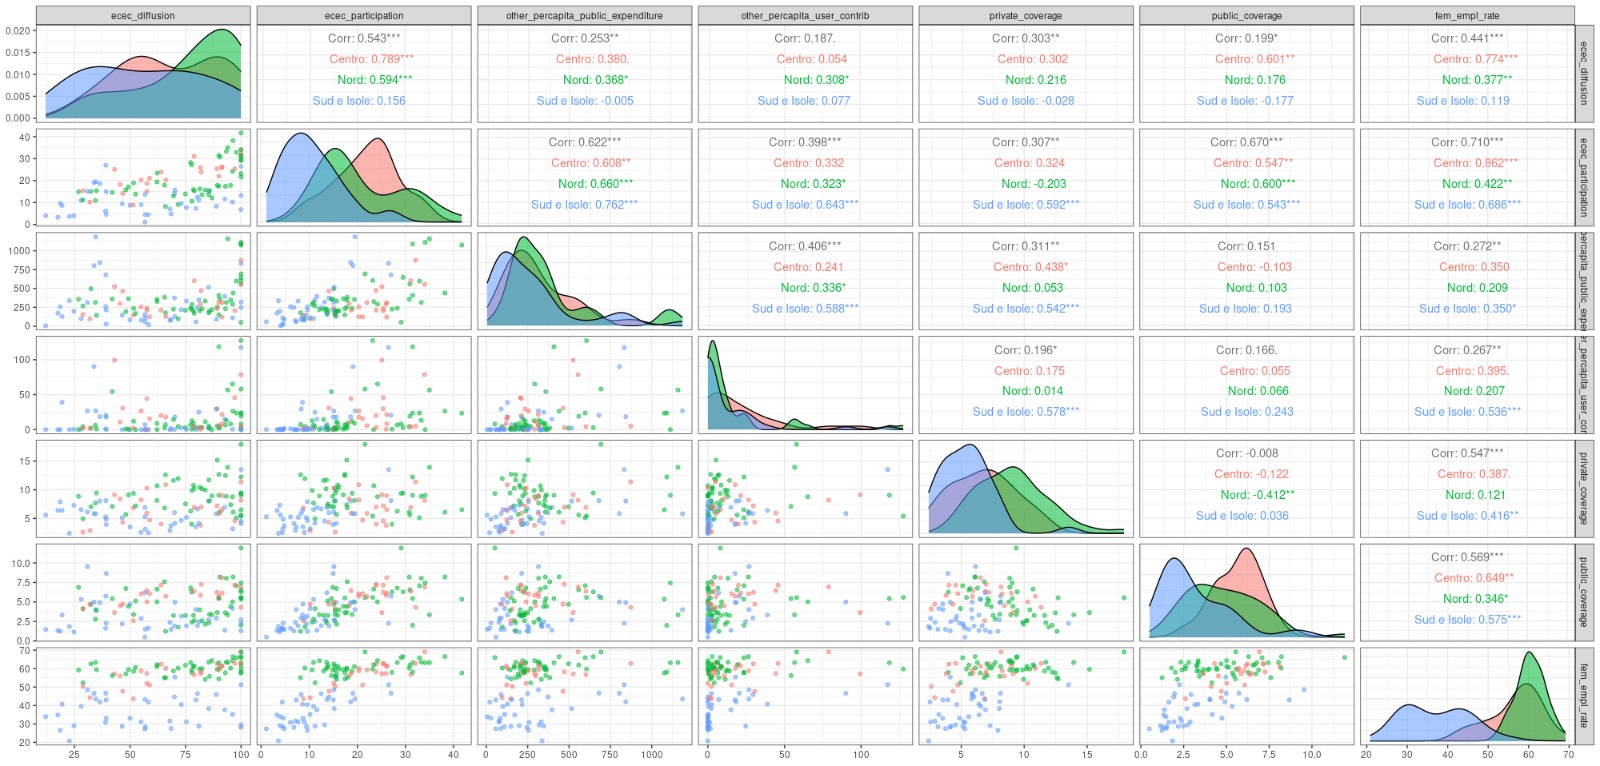
\includegraphics[width=\linewidth]{chapters/images/scatterplots.jpeg}
    \centering
    \caption{Pairwise scatterplot matrix of the main variables used in the study.\\
    \texttt{rip\_name}: Blue = South and Islands, Green = North, Red Center.\\}.
    \label{fig:scatterplot}
\end{figure}

Table~\ref{tab:vif_values} reports the VIF values of the potential covariates before performing Bayesian LASSO.

\begin{table}[h]
\centering
\caption{VIF values of potential covariates before Bayesian LASSO.}
\label{tab:vif_values}
\begin{tabular}{lc}
\hline
\textbf{variable} & \textbf{VIF} \\
\hline
ecec\_participation & 9.140282 \\
graduate\_mobility\_rate & 8.102231 \\
advanced\_business\_empl & 7.346519 \\
n\_members\_family & 6.564543 \\
ageing\_index & 6.548976 \\
public\_coverage & 4.139228 \\
first\_birth\_maternal\_age & 4.010305 \\
fem\_edu\_rate & 3.987515 \\
other\_percapita\_public\_expenditure & 3.876044 \\
avg\_children\_per\_woman & 3.464354 \\
public\_transport\_supply & 3.437207 \\
population & 3.238429 \\
GERD\_total\_intramural & 3.057367 \\
ecec\_diffusion & 2.517609 \\
lifelong\_learn & 2.359288 \\
service\_empl\_rate & 2.229131 \\
private\_coverage & 2.186444 \\
n\_self\_empl & 1.833873 \\
startup\_ratio & 1.784709 \\
other\_percapita\_user\_contrib & 1.684447 \\
fem\_maj\_empl\_rate & 1.503210 \\
elderly\_in\_care & 1.347364 \\
empl\_growth & 1.319513 \\
\hline
\end{tabular}
\end{table}
